\documentclass{article}
\usepackage{graphicx}
\begin{document}
\title{Transformations Exam: Question 24}
\author{Ana Bhattacharjee}
\date{\today}
\maketitle{}

\begin{center}
  The transformations started with a translation and then a rotation. Since a translation and rotation are both isometries, the rectangle DEFG should remain a rectangle after the transformations are applied. Proof of this can be seen in the visual below.
  \begin{figure}[!htbp]
    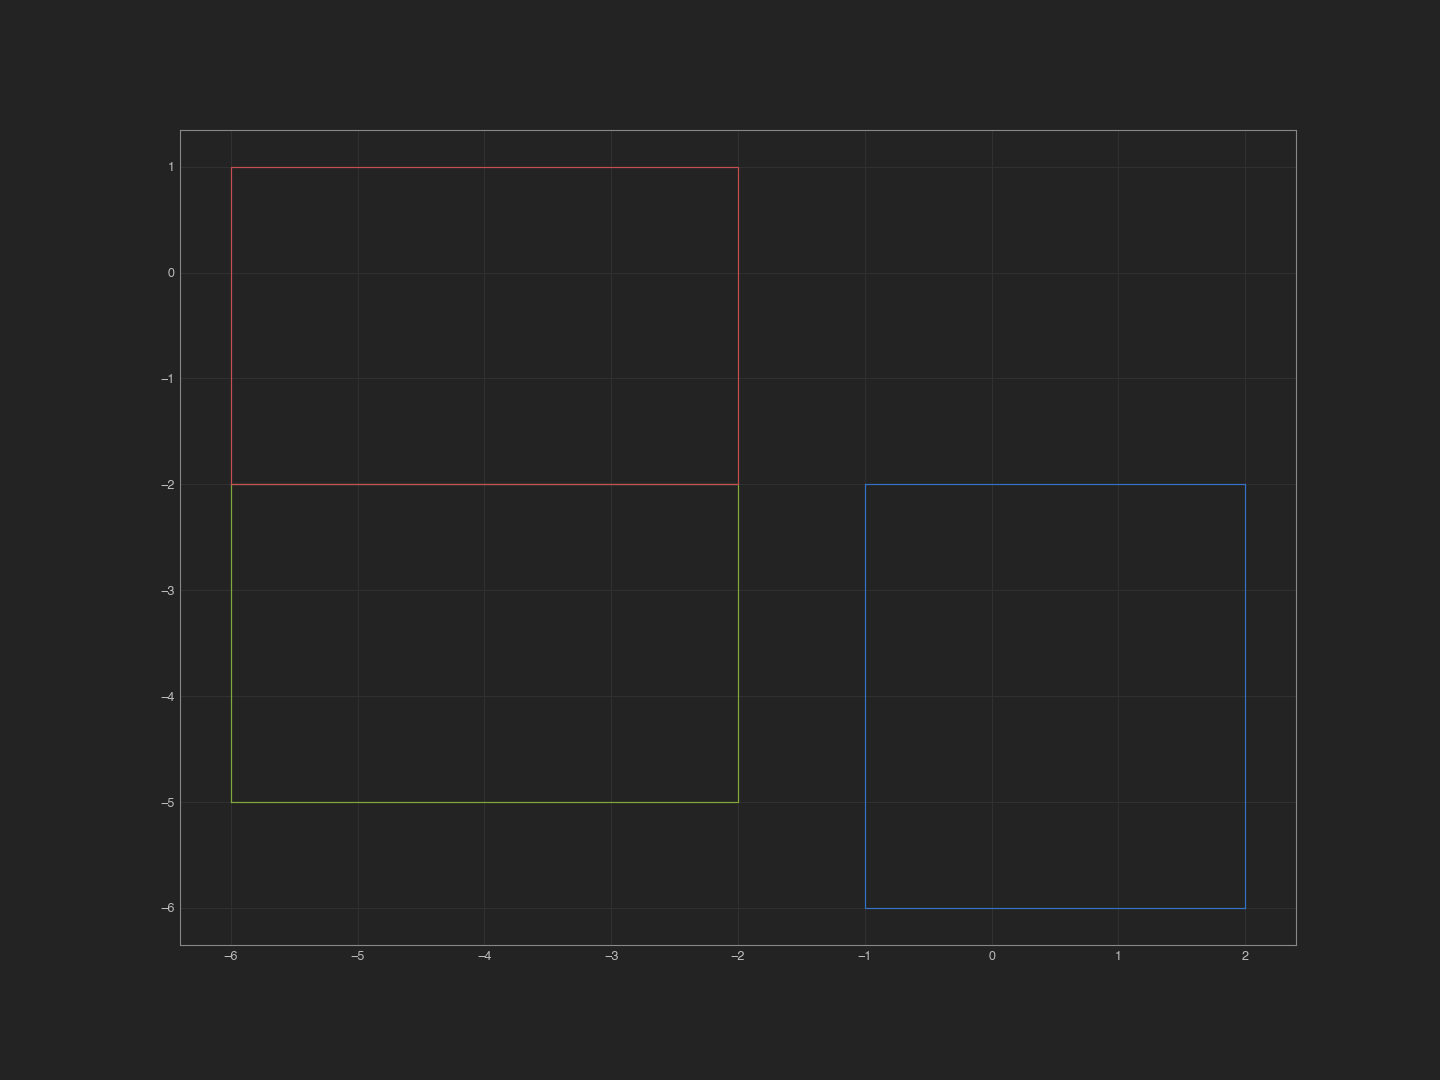
\includegraphics[width=1.0\columnwidth]{exam.png}
    \caption{Series of Transformations for Rectangle DEFG. Green (DEFG), Red (D'E'F'G'), Blue (D''E''F''G'')}
  \end{figure}
\end{center}
\end{document}
